A general multi-objective optimization problem can be described as a vector
function $f$ that maps a decision variable (solution) to a tuple
of $\np$ objectives.
Formally:
\begin{align*}
  \text{max} ~ \sol{y} &= f(\sol{x}) =
    \big(f_1(\sol{x})
    ,f_2(\sol{x})
    ,\ldots
    ,f_{\np}(\sol{x})\big) \\
  \text{subject to} ~ \sol{x} & \in X
\end{align*}
where $\sol{x}$ is the \emph{decision variable}, $X$ denotes the set
of feasible solutions, and $\sol{y}$ is the \emph{objective vector}
(or \emph{criteria vector}) where each objective has to be maximized.

Considering two decision vectors $\sol{a}, \sol{b} \in X$, $\sol{a}$ is said to
\emph{dominate} $\sol{b}$ if, and only if $\sol{a}$ is at least as good as $\sol{b}$
in all objectives and better than $\sol{b}$ in at least one objective.
For shortening we will say that $\sol{a}$ dominates $\sol{b}$ by saying $\dom{a}{b}$.
Formally:
\begin{displaymath}
    \dom{a}{b} = \left\{
      \begin{array}{l}
          \forall i \in \{1, 2, \ldots, \np\}: f_i(\sol{a}) \geq f_i(\sol{b}) ~\text{and}\\
          \exists j \in \{1, 2, \ldots, \np\}: f_j(\sol{a}) > f_j(\sol{b})
  \end{array} \right.
\end{displaymath}

A feasible solution $\sol{a} \in X$ is called \emph{efficient} %or \emph{non-dominated}
if it is not dominated by any other feasible solution.
%if there is no other feasible solution $\sol{b} \in X$ such that $\sol{b}$ dominates $\sol{a}$.
The set of all efficient solutions of a multi-objective optimization problem is
known as \emph{Pareto optimal}.
Solving a multi-objective problem consists in providing its Pareto optimal set.
It is worth remarking that the size of Pareto optimal set for this problem
tends to rapidly grow mainly with the number of objectives. 

An instance of a multi-objective knapsack problem (MOKP) with $\np$
objectives consists of an integer capacity $W > 0$ and $n$ items.
Each item $i$ has a positive weight $w_i$ and nonnegative integer
profits $p_i^1, p_i^2, \ldots, p_{i}^{\np}$.
Each profit $p_i^k$ represents the contribution of the $i$-th item for $k$-th objective.
A solution is represented by a set $\sol{x} \subseteq \{1, \ldots, n\}$
containing the indexes of the items included in the solution.
A solution is feasible if the total weight included in the knapsack does
not exceed its capacity.
Formally the definition of the problem is:
\begin{align*}
  \text{max   } & f(\sol{x}) =
    \big(f_1(\sol{x}) ,f_2(\sol{x}) ,\ldots ,f_{\np}(\sol{x})\big) \\
  \text{subject to   } & w(\sol{x}) \leq W \\
  & \sol{x} \subseteq \setIN\\
  \text{where} \phantom{mmmmm} \\
  %I_n &= \{1, \ldots, n\}\\
  f_j(\sol{x}) &= \sum_{i \in \sol{x}} p^j_i \quad j = 1, \ldots, m\\
  w(\sol{x}) &= \sum_{i \in \sol{x}} w_i
\end{align*}

The MOKP is considered a \nphard{} problem since it is a generalization
of the well-known 0$-$1 knapsack problem, in which $\np = 1$.
It is quite difficult to determine the Pareto optimal set for the MOKP,
especially for high dimensional instances, in which the
Pareto optimal set tends to grow exponentially.
Even for the bi-objective case, small problems may prove intractable.
For this reason we are interested in developing efficient methods for
handling large solution sets, which may bring tractability to previously
intractable instances.

Considering two solutions $\sol{x}, \sol{y} \subseteq \setIN$, $\sol{y}$ is
called \emph{extension} of $\sol{x}$, denoted as $\ext{y}{x}$,
iff $\sol{x} \subseteq \sol{y}$.
Any set $\sol{e} \subseteq \setIN$ such that $\sol{x} \cap \sol{e} = \emptyset$
is called an \emph{extender} of $\sol{x}$.
If $\weight{x} + \weight{e} \leq W$ than $\sol{e}$ is called a
\emph{feasible extender} of $\sol{x}$.
A solution $\sol{x}$ is called \emph{deficient} if it has available space
to fit one or more item, i.e.\,, $\weight{x} + min\{ w_i : i \notin \sol{x} \} \leq W$.
%Considering two solution $\sol{x}, \sol{y} \subseteq \setIN$
We say $\sol{x}$ \emph{knapsack-dominates} $\sol{y}$, denoted as $\domk{x}{y}$,
if $\sol{x}$ dominates $\sol{y}$ and does not weight more than $\sol{y}$.
Formally:
\begin{equation}
  \label{eq:kdom}
  \domk{x}{y} = \left\{
    \begin{array}{l}
      \dom{x}{y} \quad \text{and} \\
      w(\sol{x}) \leq w(\sol{y})
    \end{array}
  \right.
\end{equation}

The concept of knapsack dominance was proposed by Weingartner and Ness~\cite{weingartner1967methods}.
Figure~\ref{fig:kdom} illustrates the concept for a problem with $m = 1$.
Any solution in the cross-hatched area knapsack-dominates the marked solution.
The knapsack dominance concept is widely used
and is the basis of the exact algorithm
approached in Chapter~\ref{cap:kdtree}.

\begin{figure}
  \centering
  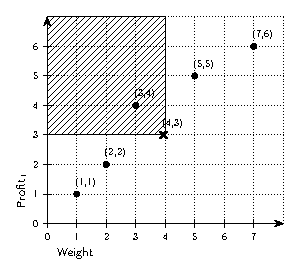
\includegraphics[scale=1.2]{img/kdt/dom}
  \caption{A knapsack-dominated solution.}
  \label{fig:kdom}
\end{figure}

